\section{架空世界における社会的決定について考える}
架空世界での社会的決定方式を考えなければいけないというのは,そもそもどういう状況なのでしょうか.例えば,創作の過程で架空世界を作ることになったとき,その世界にある王朝や国家などの共同体が,例え民主的な制度を持っていたとしても,独裁的なものだとしても,聖人君子がなんか話し合って決めごとをしているとしても,なんらかの社会的決定法があると考えるのが妥当です.そこで,どのような手法で権力者や主権者が社会的な決定を下せばいいのかという問題が生じ得ます.それも,単に独裁的に決めればいいわけではなく,合理的で人々の反感を買わないような方法でないと謀反を起こされたり,革命されちゃったりするかもしれませんし,どうすればいいのかと悩むこともあるかもしれません.

もともと,この文書を書き始めたのはそのような異世界においてどのような意思決定法が生まれてくるのだろうという疑問がきっかけでした.私自身も架空世界創作をしたことがあり\footnote{現在もしていますが.},政治レベルでの社会的決定をどうすればいいのかというのは,いまいちちゃんとした理由もなく封建制を導入したり,議会制を導入したりとしていました.

しかし,社会的決定理論の存在を知り,もしかしたらこれで架空世界の意思決定について色々と考察できるのではと考えて調べたりしました.といっても,考察にかけた時間はせいぜい二ケ月ぐらいしかないですし,具体的にどのように制度が出来上がっていくか,正当化されていくかなどと言えるほどの理解には至れませんでした.しかし,歴史的に制度が形成されていく理由を合理的に記述したりするのには役に立つ程度の知識を得ることができたとは思っています.

「投票」というと,議員選挙がイメージされるかもしれません.しかし,政治レベルに限ったとしても,法案の評決は投票ですし,最高裁の判決も投票とは言えないまでも,社会的決定の一種と言えるでしょう.つまり,社会の様々な決定プロセスへと応用が可能です.まずは実際の社会でどのような問題が起こるのかその実例について少し紹介した後に,{\bf 結局,多数決は何をしてもダメ}という本質に迫りたいと思います.

\subsubsection*{18世紀フランス科学アカデミーでの論争}
18世紀,フランス科学アカデミーという学術団体では,その会員を決めるのに単記投票方式を用いていたそうです.しかし,自身も会員だったボルダは単記投票方式には問題があるということを指摘しました.

単記投票にはどのような問題があるのでしょうか.選択肢x,y,zに対して,7人の個人$a\sim g$が図28のように選好しているとします.
\begin{figure}[!h]
    \centering
    \begin{tabular}[!h]{|c|c|c|c|c|c|c|c|} \hline
         & a & b & c & d & e & f & g \\ \hline
        1 & x & x & x & y & y & z & z \\ \hline
        2 & y & y & y & z & z & y & y \\ \hline
        3 & z & z & z & x & x & x & x \\ \hline
    \end{tabular}
    \caption{個人的選好}
\end{figure}
この時,単記投票を取ると,xが最も多く得点します.ここで,逆に最も悪いと思う選択肢はどれかと聞くと,またxが最も多く得点してしまいます.つまり,単記投票ではこの7人が最良と選択する要素と最悪と選択する要素が同じだという結果を導いてしまいます.すべての個人の選好が反転した時に社会的選好が反転前と同一であってはならないとする条件を双対性と言います.この例から単記投票は双対性を満たしていないことがわかります.

ボルダはこのような単記投票の欠陥を指摘し,1784年科学アカデミーの会員の決定方式はボルダ得点法へと変わりました.しかし,3章で説明した通り,ボルダ得点法には戦略的に結果を操作できるという欠陥があります.1800年,ナポレオン・ボナパルトによってそのことを指摘された\footnote{この欠陥を最初に指摘したのはおそらくラプラスで,ナポレオンは二番煎じです.}科学アカデミーはボルダ得点法をやめ,信任投票で会員を決めるようになったそうです.  

\subsubsection*{1955年米上院,道路建設に関する法案を巡る争い\footnote{
    この話は参考文献[1]によるが,その出典はR.Farquharson "Theory of Voting" (1969)らしいです.しかし,原著を閲覧することができず,ネットで検索してもそれらしい情報が見つからないので,信憑性に疑問はあります.誰か情報あればください.架空世界創作の参考になるかが至上命題なので掲載しました.
}}
1955年,米上院で過半を取る民主党は新国道建設法案を上院に提出しました.この時,法案には労働者に公正な賃金を払うとするデービスベーコン法を適用させる一文が盛り込まれていました.これに対して,南部出身の民主党議員からは,北部出身の民主党員による南部への干渉だとの批判が起こりました.南部民主党はデービスベーコン法に関する部分を削除した修正案を提出します.他方,共和党は新法案の撤回を求めました.原案のままでは南部民主党と共和党が反対します.修正案では北部民主党と共和党が反対します.しかし,廃案にするのは民主党の方針に合いません.困りました.

北部共和党はなんとしても法案を通過させたい.南部側はデービスベーコン法の適用だけは何がなんとしても避けたい.他方,実は共和党側は原案と修正案なら原案の方が良いと考えていたのです\footnote{なんでそうなるのかよくわかりませんが,デービスベーコン法の提出者が共和党の人だからなのかなあなどと思いました.誰か教えてください.}.つまり,各陣営の個人的選好は次のようになります.
\begin{align*}
    北部民主党 :&  原案 > 修正案 > 廃案 \\
    南部民主党 :&  修正案 > 廃案 > 原案 \\
    共和党     :&  廃案 > 原案 > 修正案
\end{align*}
よく見ると,最初の昼ご飯の例と同じです.すなわち,投票のパラドックスが生じます.

そこで,民主党の上院議員で党首だったリンドン・ジョンソンと同じく民主党の上院議員アルバート・ゴア・シニアは考えました.実はこの二人,南部出身の民主党員でした.ジョンソンとゴアはどうにかして修正案を通したいと思っていました.ジョンソンの提案で上院はまず,「原案を採択するか,修正や廃案の協議に持ち込むか」で評決を取りました.南部の民主党員と共和党員の反対で協議に入ることになりました.次に修正案か廃案かで評決を取ると,上院で過半数を取っていた民主党員が賛成したため,なんと修正案が通ってしまいました.

これは最初の昼ご飯の例で言うところの,nymwaくんの独断でラーメンを食べることに決定するのと同じです.社会的に選ばれてほしい選択肢の評決を最後に持ってくるのがポイントです.しかし,立法府たる議会でこんな独裁的な議会運営が許されてしまうというのは驚きです\footnote{誰か架空世界創作のネタで使ってください.}.

とまあ,現実でも社会的決定の困難さのせいで様々なパラドックスが生じてしまします.これが民主的な意思決定なのかというのは甚だ疑問です.一体どうすれば民主的と言えるのでしょうか.

\subsection{多数決と民主制は無関係}
先程上げた例ではいずれも単記投票方式が問題の根源となっていることがわかると思います.今までの議論からわかるように,我々が多数決として普段用いているその方式は,欠陥だらけのものだと言えます.特に単記投票では,個人的選好を完全に反映させることができない,つまり死票が多いですし,選択肢をいじれば戦略的に結果を操作でき得ます.それを改善しようとすると,個人的選好の自由を制限したり,社会的選好が循環したりすることを許さなければなりません.

じゃあ,多数決なんかやめようと,もっと根本から逆転の発想でなんとかならないか,とも思えてきます.しかし,社会の全個人の意見を聞いて社会全体の幸福度を最大限にしたり,社会全員が納得したりするような社会的決定を行うことは,その手間の多さや社会の複雑さから考えるとほとんど困難だと言えるでしょう.社会はどうしても個人的選好を入力とした関数としての社会的意思決定を執り行うことになります.そして,そのためにはどこかで社会的決定のルールを決めておかなければ混乱が生まれるだけです.安定的な社会的決定を持続的に行うためには,どこかでルールを決めそのルールにのっとって決めた社会的選好を社会が御神託として受け入れる必要があります.その御神託が奇妙で受け入れ難いものにならないようにしなくてはなりません.しかし,どうしても完璧な御神託を生み出す方式は存在しないというのがアローの不可能性定理ですし,アロー4条件を緩めてみてもいまいち良い妥協点が見つかるわけでもありませんでした.

世の中には様々な投票方式があるらしいです.それぞれがそれなりに利点・欠点を持っています.社会がどの投票方式を選択するかは,それぞれの方法の利点・欠点に依存すると考えられます.それぞれの社会が時代の要請に答えその時々に合う方法を選択して行くと考えられます.例えば,日本では55年体制の崩壊を受け1994年に衆議院議員の選挙制度が中選挙区制から小選挙区比例代表並立制へと変わりました.中選挙区では選挙にお金がかかりますし,リクルート事件などの汚職,政治腐敗などの根絶を求めた政治改革への動きが選挙制度改革の原動力となったそうです.\footnote{ただし,これは比例代表制へと向かう世界の流れと逆行するものだという批判があったり,そもそも導入した側も不本意だったみたいです.\footnotemark}.\footnotetext{http://diamond.jp/articles/-/14406}

それぞれの投票方式には個性というか,良し悪しがあります\footnote{例えばボルダ投票では全員が正直者であるときに合理的とみなせます.}.架空世界における投票方式を考えるということは,その世界での社会の状況や合理性の論理を正当化する投票方式を考えるということなのかもしれまん.ちょっと具体的に見ていきましょう.

\subsection{そうだ,多数決しよう}
多数決は個人の平等性を満たしています.さすがに個人の平等性は満たされるべきですし,多数決に限って比較していきます.

\subsubsection*{単記投票の問題まとめ}
単記投票と今まで漠然と言ってきたが,実は単記投票にもいろいろあります.今までは一回投票してもらって,一番票数が多いものが選ばれるという,いわゆる単純多数決のみを指していましたが,決選投票を行うなど様々な改良を加えたものもあります.

単純多数決には双対性がないことは今まで見たとおりです.また,選択肢xが選ばれたとしても,多くの人がxを支持しているとも言えません.そもそも半数近くの人が投票を棄権していることも考えられますし,先に見たように戦略的投票可能性の問題もあるからです.実はxを最も良いと思っているけど,xが圧勝しそうなのでバランスを取るべきだと考えて異なる選択肢yに投票するというような投票行動なども考えられます.

また,上位二人以上を選出するいわゆる大選挙区制の場合,例えば一選挙区で二人選ぶとして同率二位が発生した場合にどちらが当選するかを公平に選ぶのは難しそうです.この場合,最終的にはくじ引きで決めることになるでしょうが,それが公平と言えるかは怪しいです.決選投票やオーストラリアで行われているような選好投票をすればこの問題自体は解決されます\footnote{ただし別の問題が発生したりするので社会的決定は難しいです.}.

\subsubsection*{多数決決定法の限界まとめ}
多数決決定法は個人と選択肢の平等性を満たすという点に限れば優れた決定方式です.しかし,アローの不可能性定理,ハンソンの定理のいずれからもわかるように社会的選好が必ずしも推移性を保つものになるとは限らないことは今まで見てきたとおりです.

多数決決定法では個人の選好を制限すれば社会的な推移性を満たすことは5章で見たとおりです.実は,個人の数が奇数のとき\footnote{単峰型投票,タブー型投票など.}や,社会に推移性ではなく非循環性を要請したときはより緩い制限\footnote{価値制限,限定的同意など.}ですむのですが,いずれにせよその制限というのが結構厳しくて,個人の選好をかなり制限するものになってしまいます.

\subsubsection*{決選投票方式}
単純多数決では過半数の得票を得ていない選択肢も一位として選ばれ得ます.過半数の信任を得られない選択肢を社会的に選ぶのは有権者の不満につながりかねません.そこで,単純多数決で上位二つとなった選択肢について決選投票をする決選投票方式が用いられることがあります.代表的な例はフランス大統領選挙です.

\subsubsection*{1974年フランス大統領選挙}
フランス第19代大統領ジョルジュ・ポンピドゥーの逝去を受け1974年5月,大統領選挙が行われました.ポンピドゥー政権で首相を務めたシャバン・デルマス,経済財務省のジスカール・デスタン,郵政通信省のジャン・ロワイエが出馬と分裂.一方左派は統一候補として社会党のフランソワ・ミッテランを擁立しました.

フランス大統領選挙では一回目の投票で有効票の過半数の支持を得た候補がいなければ,二週間後に上位2名で決選投票を行うことになっています.実際の得票数は図29のようになりました.
\begin{figure}[!h]
    \centering
    \begin{tabular}[!h]{|c|c|c|} \hline
        & 一回目 & 二回目 \\ \hline
        ミッテラン & {\bf 43.25\%} & 49.19\% \\ \hline
        デスタン   & {\bf 32.60\%} & {\bf 50.81\%} \\ \hline
        デルマス   & 15.11\% & \\ \hline
        ロワイエ   & 3.17\%  & \\ \hline
    \end{tabular}
    \caption{選挙結果 \protect\footnotemark}
\end{figure}
\footnotetext{出典はhttp://www.france-politique.fr/election-presidentielle-1974.htm.有効票における得票率です.}
一回目の投票では左派統一候補のミッテランが4割以上の支持を得ましたが,決選投票ではおそらく与党支持者の票がデスタンに集まったために,デスタンが逆転して接戦を勝利しました.

さて,もしこの例で単純多数決を用いてたならば,ミッテランが勝利することになります.単にミッテランかデスタンの二択ならデスタンを選好する個人が多いからデスタンになるべきだという理由で決選投票方式は単純多数決より優れていると言えるでしょうか.

実は決選投票方式も単純多数決と同じく双対性を満たしていません.個人$a \sim h$,選択肢$u \sim z$に関して図30のような選好を考えます.

\begin{figure}[!h]
    \centering
    \begin{tabular}[!h]{|c|c|c|c|c|c|c|c|c|} \hline
          & a & b & c & d & e & f & g & h \\ \hline
        1 & x & x & x & y & y & z & z & z \\ \hline
        2 & y & y & y & u & u & y & y & y \\ \hline
        3 & u & u & u & v & v & u & u & u \\ \hline
        4 & v & v & v & w & w & v & v & v \\ \hline
        5 & w & w & w & z & z & w & w & w \\ \hline
        6 & z & z & z & x & x & x & x & x \\ \hline
    \end{tabular}
    \caption{個人的選好}
\end{figure}

この場合,一回目の投票ではxとzが同率1位で,この2つが決選投票にかけられます.決選投票では,xが3票,zが5票となり,zが当選です.しかし,zは最も悪い選択肢を単純多数決で選んだときに同率1位となる選択肢です.このことから,双対性が満たされていないことがわかります.また,個人的選好をよく吟味して考えれば社会的にyが選ばれた方が社会全体の意志と合致しているようにも思えます.

単記投票ではどうしても個人が2位以下とする選択肢の情報を得ることができません.たとえ我々の意図が優れた選択肢を選び出そうというものであっても,単記投票を用いた以上選ばれた選択肢に対して言えることは,それが他の選択肢と比べて特別であったということだけなのです.単記投票は,会議での議長を選出\footnote{ある程度適任な者ならば誰がなっても大勢に影響はないので.}したり,特徴的・風変わりな選択肢を選ぶのには適しているかもしれません.しかし,社会的に選択肢に順序を付けようとして単記投票を用いるのは,たとえ決選投票などの多少の改良を加えたとしても,ナンセンスな方式に他ならないと言わざるを得ません.

大統領選の場合,選挙の手間が膨大になりますし,決選投票法ならば当選者は国民の過半数の支持は得たと言えるので酷い方式とまでは言えないでしょう.しかし,例えば「今年出た文学作品から優秀な作品を決選投票法で決めます」というようなことをしている文学賞がもし存在すれば,かなりやばいと思って間違いないかと思われます\footnote{奇を衒うなら別ですが.}.

\subsubsection*{勝ち抜き方式}
決選投票方式では過半数を得る候補がいない時,上位2位以外の落選を確定させて上位2位から当選者を選びました.逆に過半数を得る候補がいない時,最下位の候補を落選させ,その候補を1位とする人の票は2番目に選好する人の票として数え上げて行き,過半数を取る候補が出るまで最下位の票を分配するという方法ならどうでしょう.この方法を勝ち抜き方式と言います.

勝ち抜き方式では最も良いと選好する候補だけではなく,全候補に順番を付けて投票する必要が生まれます.つまり,勝ち抜き方式は単記投票ではありません\footnote{すなわち,連記投票です.}.オーストラリアの選挙はこの方式です\footnote{実際の例はhttps://en.wikipedia.org/wiki/Swing\_(Australian\_politics)にあるので是非.}.

オーストラリアはもともと単記投票だったのですが,1918年の国政選挙のスワン選挙区で保守系政党の地方党\footnote{Country Partyの訳.}と民族党\footnote{Nationalist Partyの訳.国民党と訳そうとしたら地方党が後にNational Partyと改称してるので,敢えて重複を避けてみました.}が分裂選挙となり,革新系の労働党の候補が当選してしまいました.そのため,当時与党だった民族党が選挙方式を変えてしまったそうです.

え,そんな理由なの,と思ってしまいましたが,日本のそれも含めて考えると,選挙制度改革の動機なんて利己的なものなのだなあという気になります.

\subsubsection*{ボルダ得点法}
ボルダ得点法はすでに述べた通り,戦略的操作可能性の問題があります.実際にボルダ投票を国政選挙に使っている国というのはいくつかあって,その1つがナウルです\footnote{どうしてナウルがボルダ得点法を用いているのかはよくわかりませんでした.おそらく有権者数が少ないのでボルダ得点法がやりやすいことが一因でしょう.}.

\subsubsection*{2016年ナウル議会議員選挙}
ナウルの選挙制度は大選挙区制で,n人の候補者に1位からn位まで順位を付けて投票します.1位の人が$1$票,2位が$\frac{1}{2}$票,\dots,n位が$\frac{1}{n}$票と得点し,点が高い方から何人かが当選します\footnote{ダウドール方式と言います.}.この方法だとオリジナルのボルダ得点法よりも戦略的投票の影響が小さくなります.これは順位と得点のグラフが下に凸になっているため,線形に重み付けをする普通のボルダ得点法よりも順位の低い選択肢への選好の影響力が小さいからです(図31).

\begin{figure}[!h]
    \centering
    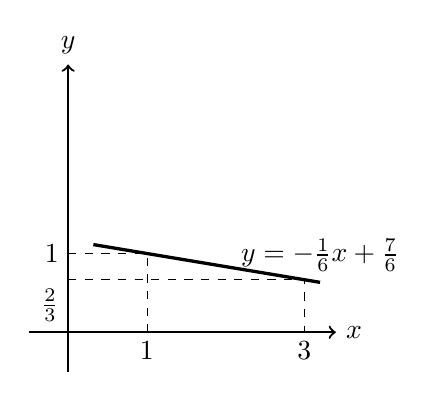
\begin{tikzpicture}[domain = 0.32:3.2, samples = 100, very thick]
        \draw[thick, ->] (-0.5, 0) -- (3.4, 0) node[right] {$x$};
        \draw[thick, ->] (0, -0.5) -- (0, 3.4) node[above] {$y$};
        \draw plot(\x, -1/6 * \x + 7/6) node[above] {$y = -\frac{1}{6}x+\frac{7}{6}$};
        \draw [very thin, dashed] (0,1) node[left]{$1$}--(1,1)--(1,0) node[below]{$1$};
        \draw [very thin, dashed] (0,0.67) node[below left]{$\frac{2}{3}$}--(3,0.67)--(3,0) node[below]{$3$};
    \end{tikzpicture}
    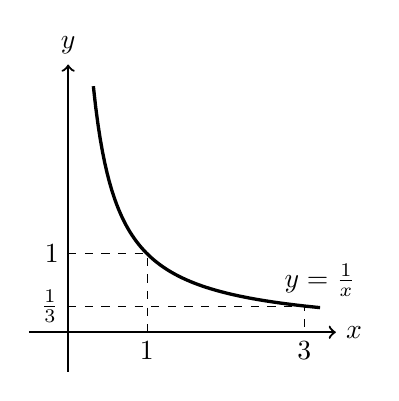
\begin{tikzpicture}[domain = 0.32:3.2, samples = 100, very thick]
        \draw[thick, ->] (-0.5, 0) -- (3.4, 0) node[right] {$x$};
        \draw[thick, ->] (0, -0.5) -- (0, 3.4) node[above] {$y$};
        \draw plot(\x, 1/\x) node[above] {$y = \frac{1}{x}$};
        \draw [very thin, dashed] (0,1) node[left]{$1$}--(1,1)--(1,0) node[below]{$1$};
        \draw [very thin, dashed] (0,0.33) node[left]{$\frac{1}{3}$}--(3,0.33)--(3,0) node[below]{$3$};
    \end{tikzpicture}
    \caption{ボルダ投票の得点重み(選択肢数は6人\protect\footnotemark)}
\end{figure}
\footnotetext{線形な重み付けで,1位の人に1票投票するとすると,候補n人中x位の人への票数$f(x)$は$f(x) = - \frac{1}{n}x + \frac{n+1}{n}$です.}

ナウルのヤレン地区での選挙結果\footnote{Wikipediaから出典を辿ろうとしたら,リンクが切れていました.Wikipedia(https://en.wikipedia.org/wiki/Nauruan\_parliamentary\_election,\_2016i)からの引用になります.}は図32のようになりました.ヤレン選挙区は定数2です.

\begin{figure}[!h]
    \centering
    \begin{tabular}[!h]{|c|c|c|c|c|c|c|c|} \hline
         & 1位 & 2位 & 3位 & 4位 & 5位 & 6位 & 得点 \\ \hline
        Scotty & 255 & 103 &  33 &  24 &  51 &  38 & {\bf 340.03} \\ \hline
        Keke   & 122 &  52 &  46 &  82 &  65 & 137 & {\bf 219.67} \\ \hline
        Eoe    &  71 & 132 &  56 &  51 &  96 &  98 & 203.95 \\ \hline
        Mackay &  11 & 119 & 128 & 123 &  82 &  41 & 167.15 \\ \hline
        Julius &  41 &  35 &  95 & 111 & 118 & 104 & 158.85 \\ \hline
        Amwano &   4 &  62 & 144 & 117 &  91 &  86 & 144.78 \\ \hline
    \end{tabular}
    \caption{ヤレン地区の開票結果}
\end{figure}

図32をよくみると,得点の高い候補は票が上位と下位に分散していて,得点の低い候補は票が中位に集中しています\footnote{同じ選挙の他の選挙区でも同様の結果となっています.}.おそらく,有力な候補というのは支持者も多い傍ら不支持者も多く,泡沫候補はどちらも少ないためにこのような結果になるのでしょう.これはもう人間の心理の問題なのでしょうがないのですが,ボルダ得点法を用いる場合は得点の重み付けを工夫しないと公正さに欠くものになってしまうと言えるでしょう.

\subsubsection*{承認投票方式}
承認投票は,全選択肢を承認する選択肢と承認しない選択肢に分類し,承認する選択肢に1票ずつ投票するという方式です.最も多くの票を得た選択肢が当選します.国連事務総長選挙などで用いられているようです\footnote{日本でも最高裁判所判事の国民審査で使われています.}.

承認投票では各個人はすべての選択肢について吟味を要求します.各選択肢も個人のちょっとした意識や投票行動の変化によって当選の可能性が大きく変動し,強力な候補が落選する可能性も高くなります.これは,承認投票は今まで見てきた投票方式よりも民意を反映しやすいということです.また,贈賄があまり意味をなしません.贈賄して自分の票数が増えても,他の候補の票数が減るわけではないからです.また,各候補に順位を付けるわけではないので,戦略的投票の影響も小さくなります.ちなみに,任意の3選択肢について二分選好になっていることにも注意してください.

そう考えるとなかなかに良さそうな方式に思えます.図33の選好について考えてみましょう.
\begin{figure}[!h]
    \centering
    \begin{tabular}[!h]{|c|c|c|c|} \hline
          & a & b & c \\ \hline
        1 & x & x & z \\ \hline
        2 & y & y & y \\ \hline
        3 & z & z & x \\ \hline
    \end{tabular}
    \caption{個人的選好}
\end{figure}
すべての個人が上位1位の選択肢までを承認した場合はxが選ばれますが,上位2位までを承認した場合はyが選ばれます.例えば事前の世論調査などで予め大体の個人的選好がわかっているときに,「選択肢が4つありますが,上位2選択肢を承認してください.それ以外は無効票とします」というような承認投票を行った場合,結果を思うように操作することもできるかもしれません.

\subsubsection*{パウロスの全員当選モデル}
今まで,様々な多数決方式を見てきました.ここで,パウロスの全員当選モデルという個人的選好に対して各投票方式を当てはめてみたいと思います.図34のパウロスの全員当選モデルでは,5選択肢と55人の個人的選好が定まっています.

\begin{figure}[!h]
    \centering
    \begin{tabular}[!h]{|c|c|c|c|c|c|c|} \hline
           & 18人 & 12人 & 10人 & 9人 & 4人 & 2人 \\ \hline
         1 & x    & y    & z    & u   & v   & v   \\ \hline
         2 & u    & v    & y    & z   & y   & z   \\ \hline
         3 & v    & u    & v    & v   & u   & u   \\ \hline
         4 & z    & z    & u    & y   & z   & y   \\ \hline
         5 & y    & x    & x    & x   & x   & x   \\ \hline
    \end{tabular}
    \caption{全員当選モデル}
\end{figure}

まず,単純多数決ではxが当選します.決選投票だとyが当選.勝ち抜き投票だとzが当選.ボルダ得点で票数を線形に重み付けした時は,x:127点,y:156点,z:162点,u:191点,v:189点でuが当選.逆比例に重み付けした時は,x:25.40点,y:25.35点,z:24.00点,u:26.50点,v:24.33点でuが当選.多数決決定法では循環が生じず,v,u,z,y,xの順に選好し,vが選ばれます.

このように,方式が異なればどの候補も当選しうるということがわかります.結局,多数決で最も好ましい選択肢を選ぶということは,とっても怪しい行いで,多数決と民主制は論理的には全く無関係なものであるというのが事実なのです.

\subsubsection*{結局}
思うに,実際に選挙方式を決めているのはその時の権力者の事情とかその時の社会情勢や民意であって,{\bf どの投票方式が良いとかそういうことではない}のです.パウロスの全員当選モデルのパラドックスが示すように,多数決による意思決定の結果は,一定の公正さはありますが,もはや御神託以外の何者でもないと言ってよいでしょう.

架空世界で社会的決定のルールを決める場合,確かに「ボルダ得点法には操作可能性がある!」や「アローの不可能性定理より完璧な投票方式は存在しない!」というような論理的な主張が影響を与えることもあるでしょう.しかし,たとえ数理的な正しさを大切にする架空世界であっても,時の権力者や政権にとって現在の選挙制度が都合が悪いということが,選挙制度が変わる理由だと考えるべきではないでしょうか.結局,架空世界での選挙制度を考えるときは,公正でない方式を正したり,民意をより反映させたりという点も大事ですが,それよりも,{\bf その時選挙制度を変える権力のある者にとって議会での議席が増えたり意思決定がしやすくなるような決定方法は何か},という点について考えなければ,自然で現実的な架空世界記述ができないように思えます.

また,集計の手間や有権者の意識なども選挙制度に反映されるでしょう.議会の議席配分なら比例代表制だと死票も少なく少数者の意見が反映されやすくあまりパラドックスも生じそうもないので良いと言えるでしょうが,結局,多数決は民主的であることと無関係なわけですし,投票による意思決定にこれと言った解はないようです.

ただ,「この方式はこの世界観と合致しているか?」,「この方式ではパラドックスが生じないか?」などということを考察すると,例えば政治制度を創作する時に根本的な部分から構築ができるし,そのような方式を取るに至る歴史も考察し記述することができると思います\footnote{もともと,これが私が社会的決定理論について調べた一番強い動機です.}.どれが良いとも言えないという事実の中で,なるべく良い方法を探そうとする苦悩はどこの世界にも存在すると思いますし,それを架空の歴史の一側面として想定するなり組み込むなりすると,政治や意思決定の制度に関する創作がよりリアルなものになるでしょうし,凝ったものができるかもしれません\footnote{この文章がそういう作り込みに役立てれば幸いです.}.

ところで,今まで見てきた投票方法は,「投票所に行って,紙にバツとか数字とかを書いて投票して,選挙管理委員の人たちが徹夜して開票作業して,翌朝に結果が出る」というようなものです.どうしても複雑な過程を踏んだり,何度も予備選挙や決選投票などをやるのは金銭的にも厳しいかもしれません.

しかし,例えば情報通信技術の進歩は,投開票の手間を省略してくれるかもしれません.情報技術が進んでいたり,その導入に積極的な架空世界もあるかもしれませんし,そのような考察は何かの役に立つと思っています.最後にそのような場合の投票がどうなるか考えてみたいと思います.

